\documentclass[t, aspectratio=169]{beamer}
\usepackage{amsmath,amsfonts,amsthm,amstext,amssymb, xcolor, tikz, pgf, mathrsfs, polynom, pifont, tabto}

% ----------------------------------------------------------
% Theme Setup

% Use Metropolis Theme
\usetheme[numbering=fraction]{metropolis}
\setbeamertemplate{blocks}[rounded][shadow=false]
\makeatletter
\setlength{\metropolis@titleseparator@linewidth}{1pt}
\makeatother

% Define Colors
\definecolor{chargerblue}{HTML}{002764}
\definecolor{chargerred}{HTML}{e02034}
\definecolor{bggray}{HTML}{d0d3d4}

% Set Colors
\setbeamercolor{title}{fg=chargerblue}
\setbeamercolor{background canvas}{bg=white}
\setbeamercolor{title separator}{fg=chargerred}
\setbeamercolor{structure}{fg=chargerblue}
\setbeamercolor{frametitle}{fg=white, bg=chargerblue}
\setbeamercolor*{normal text}{fg=chargerblue}
\setbeamercolor*{block body}{bg=bggray}
\setbeamercolor*{block title}{bg=chargerblue, fg=white}
% ----------------------------------------------------------

% ----------------------------------------------------------
% Custom Definitions, Commands, Environments, etc.

% Sets of numbers
\def\R{\mathbb{R}} % The reals
\def\N{\mathbb{N}} % The naturals
\def\Z{\mathbb{Z}} % The integers
\def\Q{\mathbb{Q}} % The rationals

% Blank space
\newcommand{\blank}[1]{\underline{\hspace{#1}}} % Blank space

% Change font colors
\newcommand{\cyan}[1]{{\color{cyan}{#1}}} % Changes font to cyan
\newcommand{\red}[1]{{\color{red}{#1}}} % Changes font to red
\newcommand{\magenta}[1]{{\color{magenta}{#1}}} % Changes font to magenta
\newcommand{\orange}[1]{{\color{orange}{#1}}} % Changes font to orange
\newcommand{\yellow}[1]{{\color{yellow}{#1}}} % Changes font to yellow
\newcommand{\violet}[1]{{\color{violet}{#1}}} % Changes font to violet
\newcommand{\green}[1]{{\color{green}{#1}}} % Changes font to green
\newcommand{\blue}[1]{{\color{blue}{#1}}} % Changes font to blue
\newcommand{\white}[1]{{\color{white}{#1}}} % Changes font to white

% Fitted inclusion symbols
\newcommand{\fp}[1]{\left({#1}\right)} % Fitted parentheses around content
\newcommand{\fb}[1]{\left[{#1}\right]} % Fitted brackets
\newcommand{\lhoi}[1]{\left({#1}\right]} % Left half-open interval
\newcommand{\rhoi}[1]{\left[{#1}\right)} % Right half-open interval
\newcommand{\set}[1]{\left\{{#1}\right\}} % Fitted braces (useful for sets)
\newcommand{\av}[1]{\left|{#1}\right|} % Fitted absolute value bars

% Augmented Matrix Environment
\newenvironment{amatrix}[1]{%
	\left[\begin{array}{@{}*{#1}{c}|c@{}}
	}{%
	\end{array}\right]
}

% Miscellaneous
\def\then{\Rightarrow}
\def\to{\rightarrow}
\def\d{^{\circ}}
\newcommand{\?}{\stackrel{?}{=}}
\newcommand{\cmark}{\text{ \ding{51}}}
\newcommand{\xmark}{\text{ \ding{55}}}

% Coordinate Plane (Four-Quadrant)
\def\coordplane {
	\begin{tikzpicture}        \draw[step=0.25cm,black,very thin,opacity=0.25] (-2.5cm, -2.5cm) grid (2.5cm, 2.5cm);
		\draw[<->,thick,black] (-2.5cm, 0) -- (2.5cm, 0) node[anchor=north west,pos=0.94,font=\scriptsize]{$x$};
		\draw[<->,thick,black] (0,-2.5cm) -- (0, 2.5cm) node[anchor=south east,font=\scriptsize,pos=0.94]{$y$};
	\end{tikzpicture}
}

% Coordinate Plane (One-Quadrant)
\def\onequad {
	\begin{tikzpicture}
		\draw[step=0.25cm, black, very thin, opacity=0.25] (0,0) grid (7.5cm,5cm);
		\draw[->, thick, black] (0,0) -- (7.5cm, 0) node[anchor=north west,font=\scriptsize,pos=0.94]{$x$};
		\draw[->, black, thick] (0,0) -- (0,5cm) node[anchor=south east,font=\scriptsize,pos=0.94]{$y$};
	\end{tikzpicture}
}
% ----------------------------------------------------------

% ----------------------------------------------------------
% Presentation Information
\title[5-1]{Probabililty Distributions; Mean of a Probability Distribution}
\subtitle{Sections 5-1 and 5-2}
\author{Jacob Ayers}
\institute{Lesson \#14}
\date{MAT 110}
% ----------------------------------------------------------

\begin{document}
	
	% Slide 1 (Title Slide)
	\begin{frame}
		\titlepage
	\end{frame}
	
	% Slide 2 (Objectives)
	\begin{frame}{Objectives}
		\begin{itemize}
			\item Construct probability distributions and their graphs
			\item Determine whether a distribution represents a probability distribution
			\item Compute the mean of a probability distribution
		\end{itemize}
	\end{frame}

	\begin{frame}{Review of Variables}
		Recall: A \textit{variable} is a characteristic that can assume different values. \pause
		
		In this chapter, we will study \textit{random variables}.
		
		\begin{block}{Random Variables}
			A \textit{random variable} is a variable whose values are determined by chance.
		\end{block} \pause
	
		Examples of random variables: \begin{itemize}
			\item Rolling a die
			\item Drawing a card from a shuffled deck
		\end{itemize}
	\end{frame}

	\begin{frame}{Review of Variables}
		Recall: Variables are either \textit{discrete} or \textit{continuous}. \pause
		
		A \textit{discrete variable} is a variable with a countable number of outcomes. \pause
		
		A \textit{continuous variable} is a variable whose possible values can be measured rather than counted. \pause
		
		Examples of discrete variables: number of athletes on the track team, number of text messages sent \pause
		
		Examples of continuous variables: weight, height, temperature \pause
		
		In Chapter 5, we will be studying probability distributions for discrete variables.
	\end{frame}

	\begin{frame}{Probability Distributions}
		To see how to construct a probability distribution, let's look at an example.
		
		Say we flip a coin, and we are interested in the number of heads that we obtain. \pause
		
		First, we can make a tree diagram to see the sample space:
	\end{frame}

	\begin{frame}{Probability Distributions}
		There is $1$ way of getting no heads, so $P(0) = \dfrac18$. \pause \\
		There are $3$ ways of getting 1 head, so $P(1) = \dfrac38$. \pause \\
		There are $3$ ways of getting 2 heads, so $P(2) = \dfrac38$. \pause \\
		There is $1$ way of getting 3 heads, so $P(3) = \dfrac18$. \pause
		
		To construct a \textit{probability distribution} for this experiment, simply put this information into a table. \pause
		
		\begin{tabular}{c|cccc}
			Number of Heads $X$ & 0 & 1 & 2 & 3 \\ \hline
			Probability $P(X)$ & $\frac18$ & $\frac38$ & $\frac38$ & $\frac18$
		\end{tabular}
	\end{frame}

	\begin{frame}{Probability Distributions}
		Here is the formal process for creating a probability distribution: \begin{enumerate}[1)]
			\item Make a frequency distribution for the outcomes of the variable. \pause
			\item Find the probability for each outcome by dividing the frequency of the outcome by the number of outcomes in the sample space. \pause
			\item If a graph is required, construct a vertical bar graph with the outcome on the horizontal axis and the probability on the vertical axis. \pause
		\end{enumerate}
	
		We can use Google Sheets to make the graphs when necessary.
	\end{frame}

	\begin{frame}{Probability Distributions}
		Construct a probability distribution for the sum of two six-sided dice, and represent it graphically. \pause
		
		First, let's draw out the sample space using a table: \pause
		
		\begin{tabular}{|c|c|c|c|c|c|c|} \hline
			 & \textbf{1} & \textbf{2} & \textbf{3} & \textbf{4} & \textbf{5} & \textbf{6} \\ \hline
			 \textbf{1} & 2 & 3 & 4 & 5 & 6 & 7 \\ \hline
			 \textbf{2} & 3 & 4 & 5 & 6 & 7 & 8 \\ \hline
			 \textbf{3} & 4 & 5 & 6 & 7 & 8 & 9 \\ \hline
			 \textbf{4} & 5 & 6 & 7 & 8 & 9 & 10 \\ \hline
			 \textbf{5} & 6 & 7 & 8 & 9 & 10 & 11 \\ \hline
			 \textbf{6} & 7 & 8 & 9 & 10 & 11 & 12 \\ \hline
		\end{tabular}
	\end{frame}

	\begin{frame}{Probability Distributions}
		We can use the sample space to create the probability distribution: \pause
		
		\begin{tabular}{c|ccccccccccc}
			$X$ & 2 & 3 & 4 & 5 & 6 & 7 & 8 & 9 & 10 & 11 & 12 \\ \hline
			$P(X)$ & $1/36$ & $1/18$ & $1/12$ & $1/9$ & $5/36$ & $1/6$ & $5/36$ & $1/9$ & $1/12$ & $1/18$ & $1/36$
		\end{tabular} \pause
	
		Next, use Google Sheets to create the graph.
	\end{frame}

	\begin{frame}{Probability Distributions}
		A convenience store sells AA batteries in packs of 2, 4, 6, and 8. The store sells 5 2-packs, 10 4-packs, 8 6-packs, and 2 8-packs over the weekend. Construct a probability distribution and draw its graph. \pause
		
		\begin{tabular}{c|cccc}
			Pack Size $X$ & 2 & 4 & 6 & 8 \\ \hline
			Probability $P(X)$ \pause & $0.20$ \pause & $0.40$ \pause & $0.32$ \pause & $0.08$ \pause
		\end{tabular}
	
		Use Google Sheets to create the graph.
	\end{frame}

	\begin{frame}{Probability Distributions}
		In order for a distribution to be a probability distribution, it must meet two requirements: \pause \begin{enumerate}[1)]
			\item The sum of the probabilities of all the events in the sample space must be 1 ($\sum P(X) = 1$) \pause
			\item The probability of each event must be between 0 and 1, inclusive ($0 \leq P(X) \leq 1$)
		\end{enumerate}
	\end{frame}

	\begin{frame}{Probability Distributions}
		Determine whether each distribution is a probability distribution:
		
		a) \begin{tabular}{c|ccccc}
			$X$ & 2 & 4 & 6 & 8 & 10 \\ \hline
			$P(X)$ & 0.3 & 0.4 & 0.1 & 0.2 & 0.1
		\end{tabular}
	
		b) \begin{tabular}{c|cccc}
			$X$ & $\spadesuit$ & $\diamondsuit$ & $\heartsuit$ & $\clubsuit$ \\ \hline
			$P(X)$ & 1/2 & 1/4 & 1/8 & 1/8
		\end{tabular}
	
		c) \begin{tabular}{c|cccc}
			$X$ & 3 & 7 & 10 & 12 \\ \hline
			$P(X)$ & -0.6 & 0.3 & 0.3 & 0.2	
		\end{tabular} \pause
	
		a) No; sum is 1.1 \pause \\ b) Yes \pause \\ c) No; negative probability + sum is 0.2
	\end{frame}

	\begin{frame}{Mean of a Probability Distribution}
		Recall: To calculate a weighted mean, use the formula $\overline{X} = \dfrac{\sum (w \cdot X)}{\sum w}$
		
		The formula for the mean of a probability distribution is a specific case of this formula. \pause
		
		The weights ($w$'s) are the probabilities, and the $X$'s are the outcomes. \pause
		
		The sum of the probabilities must be 1, so the denominator of the fraction is 1.
		
		So, to find the mean of a probability distribution, use the following formula: \begin{flalign*}
			\mu &= X_1 \cdot P(X_1) + X_2 \cdot P(X_2) + \cdots + X_n \cdot P(X_n) & \\
			&= \sum (X \cdot P(X))
		\end{flalign*} \pause
	\end{frame}

	\begin{frame}{Mean of a Probability Distribution}
		When rounding the mean of a probability distribution, use one more decimal place than is present in the outcomes. \pause
		
		Example: Find the mean of the number of spots that appear when a die is tossed. \pause
		
		Start by creating a probability distribution. \pause
		
		\begin{tabular}{c|cccccc}
			Outcome $X$ & 1 & 2 & 3 & 4 & 5 & 6 \\ \hline
			Probability $P(X)$ & 1/6 & 1/6 & 1/6 & 1/6 & 1/6 & 1/6
		\end{tabular} \pause
		Now, find the mean using the formula: \pause \begin{flalign*}
			\mu &= \sum (X \cdot P(X)) & \\
			&= 1\fp{\dfrac16} + 2\fp{\dfrac16} + 3\fp{\dfrac16} + 4\fp{\dfrac16} + 5\fp{\dfrac16} + 6\fp{\dfrac16} & \\
			&= \dfrac{21}{6} = 3.5
		\end{flalign*}
	\end{frame}

	\begin{frame}{Mean of a Probability Distribution}
		A fitness center bought a new exercise machine called the Mountain Climber. They decided to keep track of hwo many people used the machine over a 3-hour period. If $X$ is the number of people who used the machine, find the mean of the probability distribution.
		
		\begin{tabular}{c|ccccc}
			$X$ & 0 & 1 & 2 & 3 & 4 \\ \hline
			$P(X)$ & 0.1 & 0.2 & 0.4 & 0.2 & 0.1
		\end{tabular} \pause
	
		\begin{flalign*}
			\mu &= \sum (X \cdot P(X)) & \\
			&= 0(0.1) + 1(0.2) + 2(0.4) + 3(0.2) + 4(0.1) & \\
			&= 2.0
		\end{flalign*}
	\end{frame}

	\begin{frame}{Mean of a Probability Distribution}
		The leading digits in actual data, such as stock prices, population numbers, death rates, and lengths of rivers, do not occur randomly as one might expect, but instead follow a distribution according to Benford's law. Below is the probability distribution for the leading digits in real-life lists of data. Find the mean for the distribution.
		
		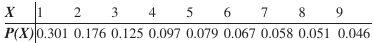
\includegraphics[width=4in]{benford.png} \pause
		
		Using a calculator: $\mu \approx 3.4$
	\end{frame}

	\begin{frame}{Next Steps}
		\begin{itemize}
			\item Read 5-2
			\item Watch Video Lesson \#15
			\item Complete Assignment \#7
		\end{itemize}
	
		\vfill
		
		Thanks for watching!
	\end{frame}
	
\end{document}